%* 
%* ------------------------------------------------------------------
%* Model Railroad System by Deepwoods Software
%* ------------------------------------------------------------------
%* AddingTrains.tex - Adding trains
%* Created by Robert Heller on Tue Mar  5 08:39:50 2002
%* ------------------------------------------------------------------
%* Modification History: $Log$
%* Modification History: Revision 1.1  2002/11/09 21:21:07  heller
%* Modification History: Time Table User Manual
%* Modification History:
%* ------------------------------------------------------------------
%* Contents:
%* ------------------------------------------------------------------
%*  
%*     Model RR System, Version 2
%*     Copyright (C) 1994-2002  Robert Heller D/B/A Deepwoods Software
%* 			51 Locke Hill Road
%* 			Wendell, MA 01379-9728
%* 
%*     This program is free software; you can redistribute it and/or modify
%*     it under the terms of the GNU General Public License as published by
%*     the Free Software Foundation; either version 2 of the License, or
%*     (at your option) any later version.
%* 
%*     This program is distributed in the hope that it will be useful,
%*     but WITHOUT ANY WARRANTY; without even the implied warranty of
%*     MERCHANTABILITY or FITNESS FOR A PARTICULAR PURPOSE.  See the
%*     GNU General Public License for more details.
%* 
%*     You should have received a copy of the GNU General Public License
%*     along with this program; if not, write to the Free Software
%*     Foundation, Inc., 675 Mass Ave, Cambridge, MA 02139, USA.
%* 
%*  
%* 

\chapter{Adding Trains}
\label{chapt:AddingTrains}

To add a train you click on the {\tt New Train} button.  This causes the
``Create New Train'' dialog box to be displayed, as shown in
Figure~\ref{fig:createNewTrainDialog}.  This dialog box collects the
basic information about the train, such as its number, section (if any),
name (if it has one), its speed in $smph$ or $skph$, as described
in Section~\ref{sect:GettingStationList}, on
page~\pageref{sect:GettingStationList}, and the trains class, as well as
the train's originating and terminating stations.

\begin{figure}
\begin{centering}
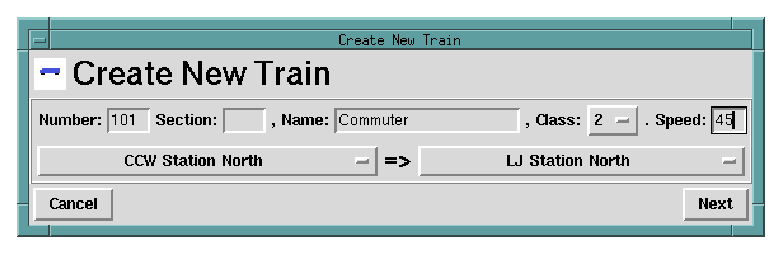
\epsfig{file=TimeTable/createNewTrainDialog.ps}\\
\caption{Create New Train Dialog box.}
\label{fig:createNewTrainDialog}
\end{centering}
\end{figure}   

Once you have entered the basic information for the train, an initial
train schedule is displayed with the ``Get Train Schedule'' dialog box,
as shown in Figure~\ref{fig:getTrainScheduleDialog}.  Initially, the
train is set to depart at midnight and make no stops and be drawn in
black (or the first cab in the (alphabetical) cab list).  The departure
times and cab/color can be changed and the {\tt Update} button clicked
on.  You can allow for layout times (for switching, etc.) by increasing
the departure time from the computed value.  Again clicking the {\tt
Update} button propagates the changes down the schedule.  Clicking {\tt
Finish} will take you to the storage track selection for departure and
arrival, if there are storage tracks at the storage tracks at the
originating or terminating stations.

\begin{figure}
\begin{centering}
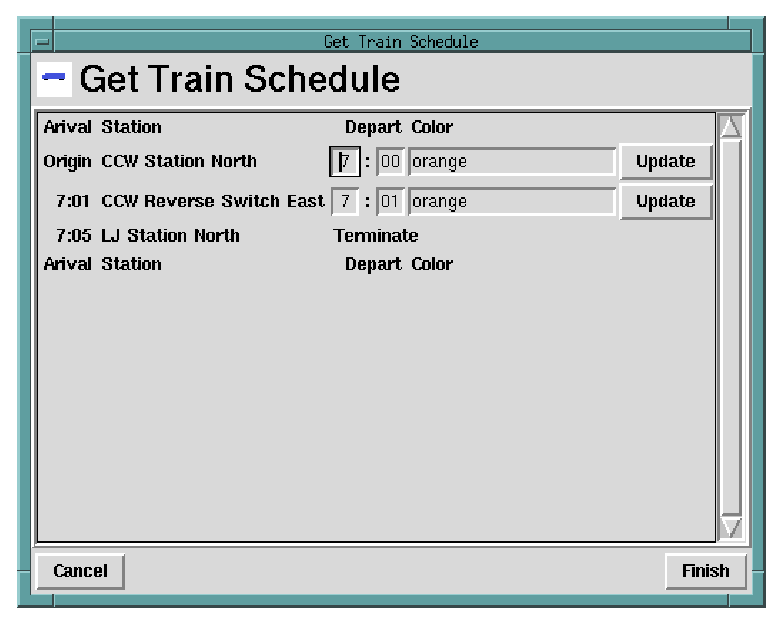
\epsfig{file=TimeTable/getTrainScheduleDialog.ps}\\
\caption{Get Train Schedule Dialog box.}
\label{fig:getTrainScheduleDialog}
\end{centering}
\end{figure}



